\section{title}

\subsection{subsection}

a equation
$$
p(y=c|x, w) = softmax(f(x))
$$
. The $w$ is the parameters of a neural network, and $f$ is the output of the model. So for each input image, we can get a probability vector $p(y=c|x, w)$.

The authors evaluated the models on MNIST~\cite{mnist}, CIFAR-10 \cite{cifar10}, a diabetic retinopathy dataset \cite{retinopathy} and ImageNet\cite{resnet}. Shaded areas in the plots denote $\pm$ one standard deviation.


\begin{enumerate}
    \item MNIST: The network architecture for MNIST, referred to as “S-CNN”
    \item CIFAR-10: The authors experiment a CNN model 
    
    Additionally they also evaluate with DenseNet-121 
    \item diabetic retinopathy dataset: Details for the inceptionV3 architecture are described in section 4.5.
    \item ImageNet: ResNet-50\cite{resnet} is used in the experiments. The network is trained for 100 epochs without data augmentation
\end{enumerate}

Figure.\ref{figure1} is show below:

\begin{figure}[ht!]
    \centering
    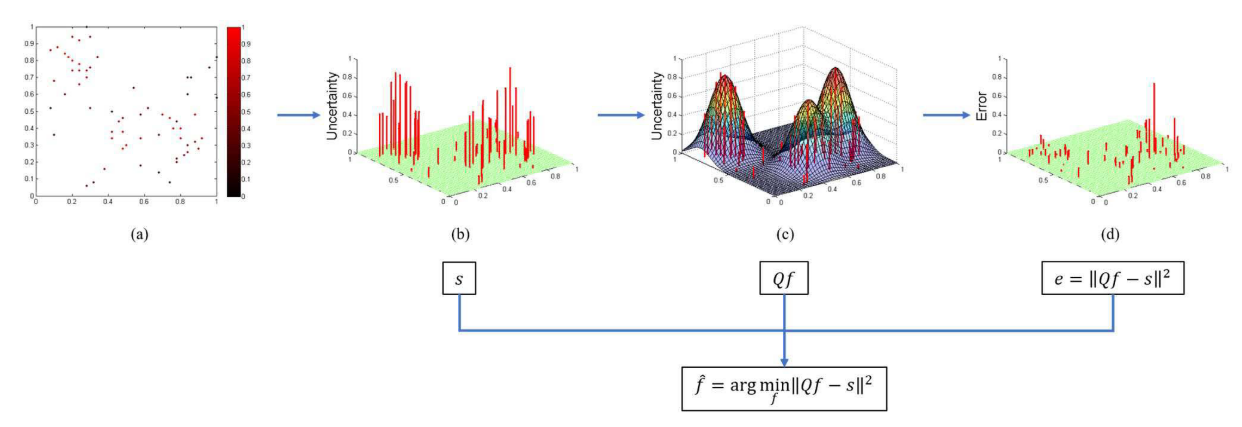
\includegraphics[width=15.4cm]{sparse_overview.png}
    \caption{overview}
    \label{figure1}
\end{figure}